\chapter{Specimen Collection}

The \entitytarget{Participant} aggregate records specimens collected
from study participants. Before specimen collection can be used, the
participant must be created. Participants cannot be added to a
\entitylink{Study} that is not enabled.

Figure \ref{fig:participant-aggregate} shows the composition of this aggregate.
A participant has a unique identifier that is used to identify the participant
in the system. This identifier is not the same as the
\valobjlink{ParticipantId} value object used by the domain model.


\begin{figure}[H]
  \centering
  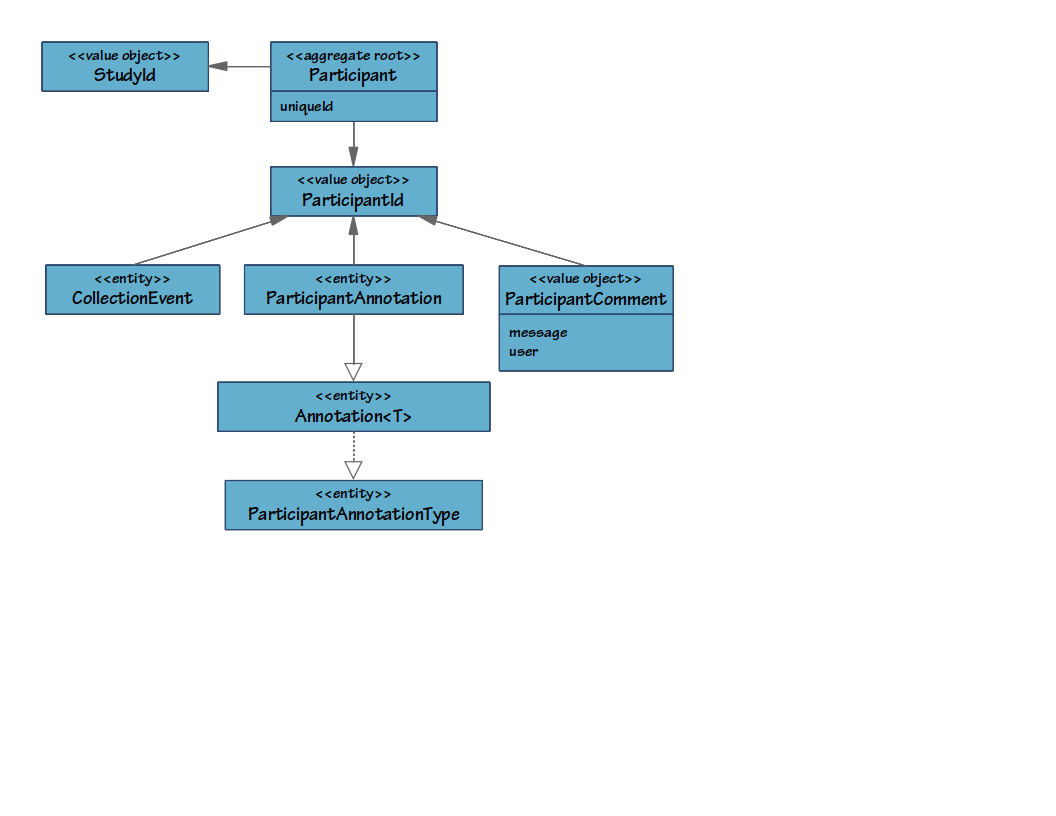
\includegraphics[trim={10mm 75mm 102mm 10mm}, clip,
    width=0.75\textwidth]{images/participant-aggregate}
  \caption{Participant aggregate}
  \label{fig:participant-aggregate}
\end{figure}

\subsection*{CollectionEvent}
Represents a visit made by a \entitylink{Participant} during which
\entitylink{Specimen}s may have been collected and other information may have
been recorded.

\subsection*{ParticipantAnnotation}
This entity holds the annotation value for the
\entitylink{ParticipantAnnotationType} defined in the study. For a single
annotation, the \emph{Value Field} used (i.e. \compfont{stringValue},
\compfont{numberValue}, or \compfont{selectedValue}) depends on the annotation
type's \compfont{valueType} (see Section \ref{sec:study-annotations}). The
unused fields are assigned the \compfont{null} value.

\begin{table}[!htbp]
\renewcommand{\arraystretch}{1.1}
\begin{tabularx}{\textwidth}{l l}
  \sffamily{\textbf{ValueType}} & \sffamily{\textbf{Value field}}\\
  \hline
  String & \compfont{stringValue}\\
  Number & \compfont{numberValue}\\
  Date & \compfont{numberValue} and stored as the number of seconds\\
  Select & \compfont{selectedValue}\\

\end{tabularx}
\end{table}

\subsection*{ParticipantComment}
A \entitytarget{ParticipantComment} contains a textual message and the user
that added the comment. The date and time the comment was made is recorded as
meta data. A participant can have one or more comments.

\section{CollectionEvent Details}

The \entitytarget{CollectionEvent} is used to record a visit to a
\entitylink{Center} (e.g. a clinic) by one of the study's participants. A
collection event must have a \entitylink{CollectionEventType} as defined by
the study. See Section \ref{sec:collection-event-type} for more details on
the collection event type.

A collection event also has a \compfont{visitNumber} that is an integer and a
\compfont{timeDone} which is a time stamp for when the participant made the
visit to the center. The format for the time stamp is: YYYY-MM-DD HH:MM.

\begin{figure}[H]
  \centering
  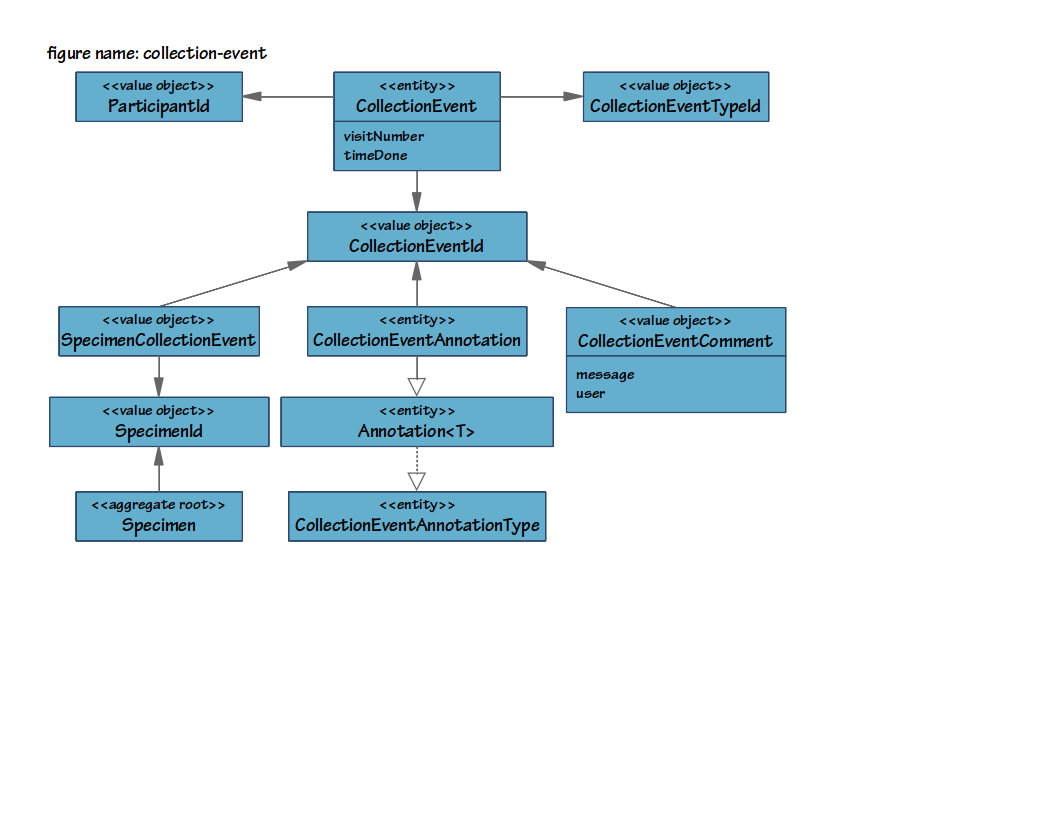
\includegraphics[trim={10mm 66mm 75mm 10mm}, clip,
    width=0.85\textwidth]{images/collection-event}
  \caption{CollectionEvent entity}
  \label{fig:collection-event}
\end{figure}

\subsection*{Specimen}
One or more specimens may have been collected from the participant. Each
specimen is recorded with the collection event. More information for this
entity is given in Section \ref{sec:specimen}.

\valobjtarget{SpecimenCollectionEvent} is used to associate a specimen to a
collection event. It is possible, although not recommended, that a specimen
have multiple collection events for the case when specimens are trasnferred
from one study to another. By having multiple collection events the information
from the original collection event is not lost for the specimen.

\subsection*{CollectionEventAnnotation}
This entity holds the annotation value for the
\entitylink{CollectionEventTypeAnnotationType} defined in the study. This field
is similar to the \entitylink{ParticipantAnnotation}. See above for how it used.

\subsection*{CollectionEventComment}
A \entitytarget{CollectionEventComment} contains a textual message and the user
that added the comment. The date and time the comment was made is recorded as
meta data. A collection event can have one or more comments.


% Local Variables:
% compile-command: "/usr/bin/rubber --pdf main"
% End:

